\documentclass[12pt]{article}

\usepackage{amsmath}
\usepackage{amsthm}
\usepackage{amsfonts}
\usepackage{amssymb}
\usepackage{tikz}
\usepackage{comment}
\usepackage{enumitem}

\setlength{\headheight}{16pt}

\topmargin=-0.25in
\evensidemargin=0in
\oddsidemargin=0in
\textwidth=6.5in
\headsep=0.25in

\linespread{1.1}
\setlength\parindent{0pt}
\setlength{\parskip}{1em}

\usetikzlibrary{shapes.geometric,fit}
\usetikzlibrary{automata,positioning}

\usepackage{fancyhdr}
\pagestyle{fancy}
\chead{CS 418: Theory of Computation \\ Homework 0}
\rhead{}

\begin{document}

\begin{flushright}Winter 2024 Version 1.0\end{flushright}

\begin{enumerate}[itemsep=1em]

\item{Even and Odd Proofs}
\begin{enumerate}
    \item Prove that the sum of two odd integers is even.
    \item Prove that the product of two even integers is even.
\end{enumerate}

\item{Polynomials}
\begin{enumerate}
    \item Determine the degree of the polynomial $p(x) = 3x^3 - 2x + 1 - 0$.
    \item Determine the degree of the polynomial $p(x) = 0x^3 - x + 2 -3$.
\end{enumerate}

\item{Sets}
\begin{enumerate}
    \item Provide an example of two sets $A, B$ where that $A$ is a subset of $B$, but $A$ is not a proper subset of $B$.
    \item Using set-builder notation, describe the set of all prime numbers less than 20.
\end{enumerate}

\item{Let $f : X \rightarrow Y$ be a function defined by the
    diagram below. 

    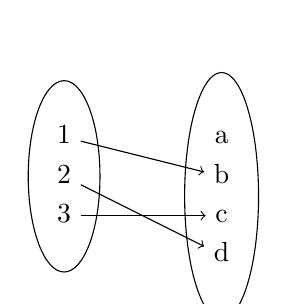
\begin{tikzpicture}
        \foreach[count=\i] \lseti/\lsetmi in {A/{1,2,3},B/{a,b,c,d}} {
            \begin{scope}[local bounding box=\lseti, x=2cm, y=0.5cm]
            \foreach[count=\j] \lj in \lsetmi {
                \node[minimum width=1em,anchor=base,text height=1.4ex,text depth=0.25ex] (n-\j-\lseti) at (\i,-\j) {\lj};
            }
            \end{scope}
            \node[ellipse, draw, fit=(\lseti)]  {};
        }
        \draw[->] (n-1-A) -- (n-2-B);
        \draw[->] (n-2-A) -- (n-4-B);
        \draw[->] (n-3-A) -- (n-3-B);
    \end{tikzpicture}

    \begin{enumerate}
        \item In terms of elements from Y, write $f(1), f(2), \text{ and } f(3)$.
        \item Represent $f$ as a set of ordered pairs.
        \item Is $f$ an injection?
        \item Is $f$ a surjection?
        \item Is $f$ a bijection?
    \end{enumerate}
    }

\newpage

\item{Graph Theory}
\begin{enumerate}
    \item Use tikz to draw a directed graph with 4 vertices and 6 edges. This must not be a hand-drawn graph.
    \item Is the graph from part (a) strongly connected? Justify your answer.
\end{enumerate}


\item{An \textbf{alphabet} is a nonempty, finite set. Which of the following are alphabets? Write True or False for each. Justify False answers.}
\begin{enumerate}
    \item{The set of all integers.}
    \item{$\{0, 1\}$}
    \item{$\{\texttt{a}, \texttt{b}\}$}
    \item{$\{x \in \mathbb{Z} : x \le 10\}$}
    \item{$\emptyset$}
\end{enumerate}
\item{A \textbf{string over an alphabet} is a finite sequence of symbols from that alphabet. Which of the following are valid strings over alphabets? Write True or False for each. Justify False answers.}
\begin{enumerate}
    \item{\texttt{0101}, over the alphabet $\{a,b\}$.}
    \item{\texttt{0a1b} over the alphabet $\{a,b\}$.}
    \item{$\varepsilon$ over the alphabet $\{a,b\}$.}
\end{enumerate}


\end{enumerate}
\end{document}
